\documentclass{standalone}
\usepackage{tikz}
\usepackage{ctex,siunitx}
\usepackage{tkz-euclide}
\usepackage{amsmath}
\usetikzlibrary{patterns, calc}
\usetikzlibrary {decorations.pathmorphing, decorations.pathreplacing, decorations.shapes}
\tikzset{
  boat/.pic={
    \fill[line join=round,gray,draw](-0.1,-0.1)--(0.1,-0.1)[bend right=30]to(0,0.4)[bend right=30]to cycle;
    \fill[line join=round,darkgray,draw](-0.08,0)--(0.08,0)[bend right=20]to(0,0.32)[bend right=20]to cycle;
  }
}
\begin{document}
\small
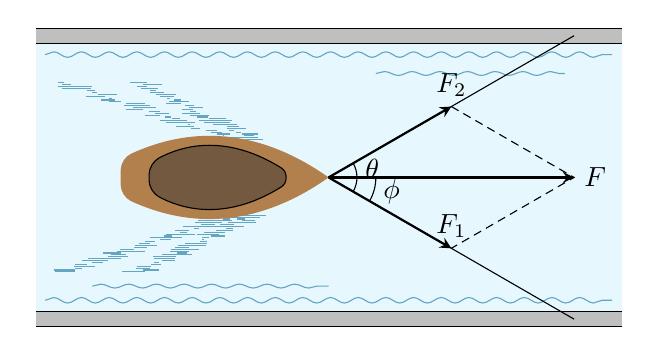
\begin{tikzpicture}[>=stealth,scale=1.2]
  % \useasboundingbox (-0.1,0.1) rectangle(6.1,-3.1);
  \fill[fill=cyan!10](-1.1,0) rectangle(5.1,3);
  \foreach \x in {0,1,...,30} 
  {
    \draw[gray!50!cyan](-0.8+\x*0.06,2.5-\x*0.02)--++(0.2*rand,0)(-0.8+\x*0.06,2.5-\x*0.02)--++(-0.2*rand,0);
    \draw[gray!50!cyan](-0.8+\x*0.06,0.5+\x*0.02)--++(0.2*rand,0)(-0.8+\x*0.06,0.5+\x*0.02)--++(-0.2*rand,0);
    \draw[gray!50!cyan](\x*0.04,2.5-\x*0.02)--++(0.2*rand,0)(\x*0.04,2.5-\x*0.02)--++(-0.2*rand,0);
    \draw[gray!50!cyan](\x*0.04,0.5+\x*0.02)--++(0.2*rand,0)(\x*0.04,0.5+\x*0.02)--++(-0.2*rand,0);
  }
  \draw[double=lightgray,double distance=5pt](-1.1,0)--(5.1,0)(-1.1,3)--(5.1,3);
  \draw[decorate,decoration={snake,amplitude=1pt}, gray!50!cyan](-1,2.8)--(5,2.8);
  \draw[decorate,decoration={snake,amplitude=1pt}, gray!50!cyan](-1,0.2)--(5,0.2);
  \draw[decorate,decoration={snake,amplitude=.7pt},gray!50!cyan](2.5,2.6)--(4.5,2.6);
  \draw[decorate,decoration={snake,amplitude=.7pt},gray!50!cyan](-0.5,0.35)--(2.0,0.35);
  \fill[brown!80!gray,rounded corners](2,1.5)to[bend right](-0.2,1.7)--(-0.2,1.3)[sharp corners]to[bend right]cycle;
  \filldraw[rounded corners,brown!40!darkgray,draw=black](1.5,1.6)to[bend right](0.1,1.65)--(0.1,1.35)[sharp corners]to[bend right](1.5,1.4)to[bend right=60]cycle;
  \draw[thick,->](2,1.5)--++(2.598,0)node[right]{$F$};
  \draw[thick,->](2,1.5)--++(30:1.5)node[above]{$F_2$};
  \draw[thick,->](2,1.5)--++(-30:1.5)node[above]{$F_1$};
  \draw[thin]([shift=(-30:0.3)]2,1.5)arc(-30:30:0.3)node[pos=0.8,right]{$\theta$};
  \draw[thin]([shift=(-30:0.5)]2,1.5)arc(-30:0:0.5)node[pos=0.4,right]{$\phi$};
  \draw[thin,densely dashed]([shift=(30:1.5)]2,1.5)--(4.598,1.5)--([shift=(-30:1.5)]2,1.5);
  \draw[thin](2,1.5)--++(30:3);
  \draw[thin](2,1.5)--++(-30:3);
  
\end{tikzpicture}
\end{document}